% Skema metode cosine dosen (tanpa contoh angka): V -> weak V1 dan strong V2 -> Head.
% Kompilasi (dari folder ini): pdflatex cosine_skema.tex && pdftoppm -png -r 300 -singlefile cosine_skema.pdf cosine_skema
\documentclass[border=6pt]{standalone}
\usepackage{amsmath}
\usepackage{amssymb}
\usepackage{mathptmx}
\usepackage{tikz}
\usetikzlibrary{arrows.meta, calc, positioning}

\definecolor{ink}{HTML}{3A3936}
\definecolor{muted}{HTML}{8A8984}
\definecolor{dataF}{HTML}{F0EFEC}
\definecolor{modelE}{HTML}{2A78D6}\definecolor{modelF}{HTML}{DCE9F9}
\definecolor{augE}{HTML}{EB6834}\definecolor{augF}{HTML}{FDE3D6}

\tikzset{
  every node/.style={font=\normalsize, text=ink, align=center},
  base/.style={rectangle, rounded corners=4pt, line width=0.9pt, inner sep=6pt},
  op/.style={base, text width=62mm, minimum height=18mm},
  weak/.style={op, draw=modelE, fill=modelF, line width=1.3pt},
  strong/.style={op, draw=augE, fill=augF, line width=1.3pt},
  head/.style={base, draw=muted, fill=dataF, text width=16mm, minimum height=58mm},
  flow/.style={-{Stealth[length=3mm]}, line width=1.2pt, draw=ink, rounded corners=6pt},
  tag/.style={font=\footnotesize\itshape, text=muted},
}

\renewcommand{\arraystretch}{1.3}
\begin{document}
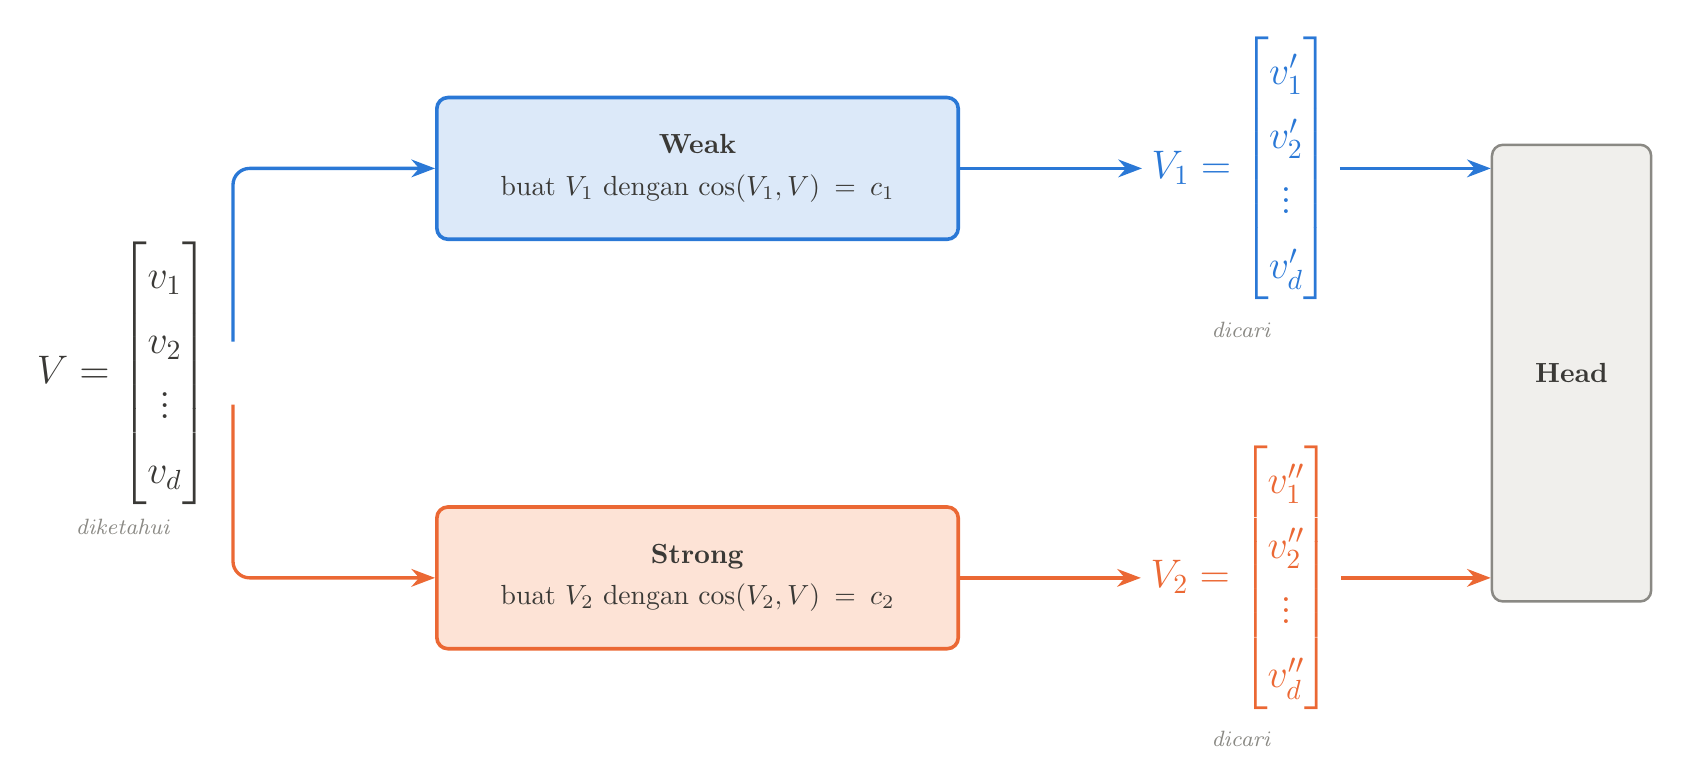
\begin{tikzpicture}

% vektor asli
\node[font=\Large] (V) at (0,0) {$V=\begin{bmatrix}v_1\\v_2\\\vdots\\v_d\end{bmatrix}$};
\node[tag] at (0,-1.95) {diketahui};

% operator weak dan strong
\node[weak]   (w) at (7.3, 2.6) {\textbf{Weak}\\[3pt]buat $V_1$ dengan $\cos(V_1,V)=c_1$};
\node[strong] (s) at (7.3,-2.6) {\textbf{Strong}\\[3pt]buat $V_2$ dengan $\cos(V_2,V)=c_2$};

% hasil
\node[font=\Large, text=modelE] (V1) at (14.2, 2.6) {$V_1=\begin{bmatrix}v'_1\\v'_2\\\vdots\\v'_d\end{bmatrix}$};
\node[font=\Large, text=augE]   (V2) at (14.2,-2.6) {$V_2=\begin{bmatrix}v''_1\\v''_2\\\vdots\\v''_d\end{bmatrix}$};
\node[tag] at (14.2, 0.55) {dicari};
\node[tag] at (14.2,-4.65) {dicari};

% head
\node[head] (h) at (18.4,0) {\textbf{Head}};

% alur
\draw[flow, modelE] (1.4,0.4) |- (w.west);
\draw[flow, augE]   (1.4,-0.4) |- (s.west);
\draw[flow, modelE] (w.east) -- (V1.west |- w.east);
\draw[flow, augE]   (s.east) -- (V2.west |- s.east);
\draw[flow, modelE] (V1.east) -- (V1.east -| h.west);
\draw[flow, augE]   (V2.east) -- (V2.east -| h.west);

\end{tikzpicture}
\end{document}
